%-------------------------------LATEX SYNTAX----------------------------------
%
%   enter:              \\, \linebreak, \newline
%   new page:           \newpage
%   tab:                \tab
%   new section:        \section{name} text
%   new paragraph       \subsection{name} text  (subsub...section{name} for more layers)
%   refer:              \nameref{label name}    (place "\label{name}" at the position you want to refer to)
%   %, &, $, etc:       \%, \&, \$, etc     (these are latex operators, add a "\" to type it as text)
%   add comment:        \commred{text}, \commblue{text}, \commpurp{text}, \commgreen{text}
%   bullet points:      \begin{itemize} \item{text} ... \item{text} \end{itemize}
%   clean code:         \cleancode{text}
%   idem without indent:\cleanstyle{text}
%   bold, italic, under:\textbf{text}, textit{text}, \underline{text}
%   table:              \begin{tabular}{c c c} text \end{tabular}   ('&' for tab, '\\' for new line)
%   
%   use Google for the rest
%   
%------------------------------------------------------------------------------

\documentclass[a4paper]{article}
\usepackage[letterpaper, margin=1in]{geometry}
\usepackage{amsmath}
\usepackage{graphicx}
\usepackage{hyperref}
\usepackage{titling}
\usepackage{float}
\usepackage[utf8]{inputenc}
\usepackage{xcolor}
\usepackage{listings}
\usepackage{easylist}
\usepackage{minted}
\usepackage{tabularx}
\usepackage{amsmath}

\definecolor{lightgray}{gray}{0.9}
\pretitle{%
  \begin{center}
  \LARGE
  
\includegraphics[width=6cm,height=6cm]{images/logo}\\[\bigskipamount]
}
\posttitle{\end{center}}
\setlength{\parindent}{0cm}

\begin{document}

\title{\Huge User Manual\\Version 2.00}
\author{\\\\\\\\\\\\\\\\\\\\\\\\\\\\\\Distributed by the Potoff and Schwiebert Groups\\\textcopyright Wayne State University}

\maketitle
\thispagestyle{empty}
\newpage

\tableofcontents
\newpage

\section{Tutorial Overview}
This document will instruct a new user how to download, compile, and run the GOMC molecular simulation code.  A basic understanding of statistical physics is recommended to complete this tutorial.\\\\
To demonstrate the capabilities of the code, the user is guided through the process of downloading and compiling a GOMC executable.  That executable is then used to perform saturated vapor and liquid equilibria (VLE) studies on systems of pure isobutane (R600a), a branched alkane that whose application as a refrigerant/propellant is increasing.\\\\
\url{http://en.wikipedia.org/wiki/Isobutane}\\\\
The Transferable Potentials for Phase Equilibria (TraPPE) united atom (UA) force field is used to describe the molecular geometry constraints and the intermolecular interactions.

\section{Introduction}
Monte Carlo (MC) simulation is a type of simulation driven by stochastic processes.  "GO" stands for GPU-Optimized; this code was intended to run optimally on modern graphics process hardware.\\\\
More specifically, this engine includes serial and GPU-Optimized (multi-threaded) codes designed to run Markov chain Boltzmann sampling of chemical systems -- effectively sets of points defined by topological maps and interaction algorithms in a simulation box.  From statistical mechanics, we know this is one way to sample phase space and model chemical systems.\\\\
GOMC currently supports canonical, isobaric-isothermal, Grand canonical, constant volume Gibbs ensemble, and constant pressure Gibbs ensemble simulations.  GOMC employs widely-used simulation file types (PDB, CHARMM-style parameter file, PSF).  GOMC includes configurational bias algorithms for both linear and branched charged, and none charged systems. 

\section{How to get the software}
The latest public code builds, project logo, manual, and other resources can be obtained via the following website:\\\\
\url{http://gomc.eng.wayne.edu/}

\begin{figure}[H]
\centering

\includegraphics[scale=0.15]{images/website}
\end{figure}

The code can be found under the download tab, below and to the right of the logo.  When new betas (or release builds) are announced, they will replace the prior code under the downloads tab.  An announcement will be posted on the front page to notify users. \\\\
Currently, version control is handled through the GitHub repository.  The posted builds in Master branch are ``frozen" versions of the code that have been validated for a number of systems and ensembles. Other branches are created as a means of implementing new features. The latest updated code builds, project logo, manual, example files, and other resources can be obtained via the following GitHub repository:\\\\
\url{https://github.com/GOMC-WSU}

\begin{figure}[H]
\centering
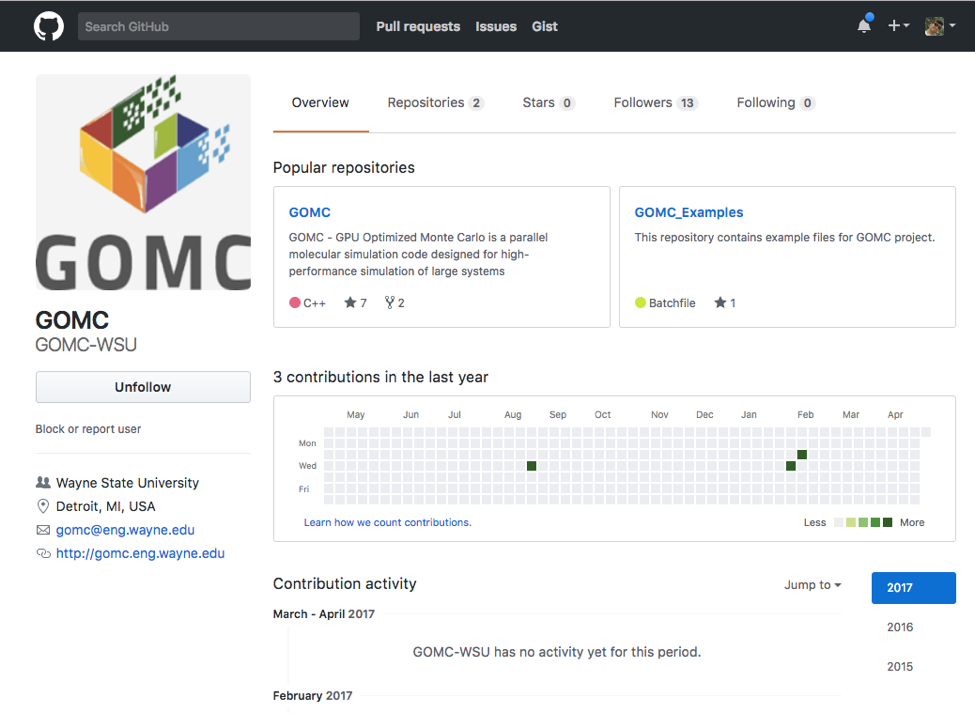
\includegraphics[scale=0.6]{images/github}
\end{figure}

The CPU and GPU code are merged together under GOMC repository and can be found under the main page. In addition, Examples repository can be found under the main page. Under each repository, the code and manual can be downloaded by clicking on the Clone or download tab. For more information regarding GitHub, visit the following link:\\\\
\url{https://guides.github.com/activities/hello-world/}

\begin{figure}[H]
\centering
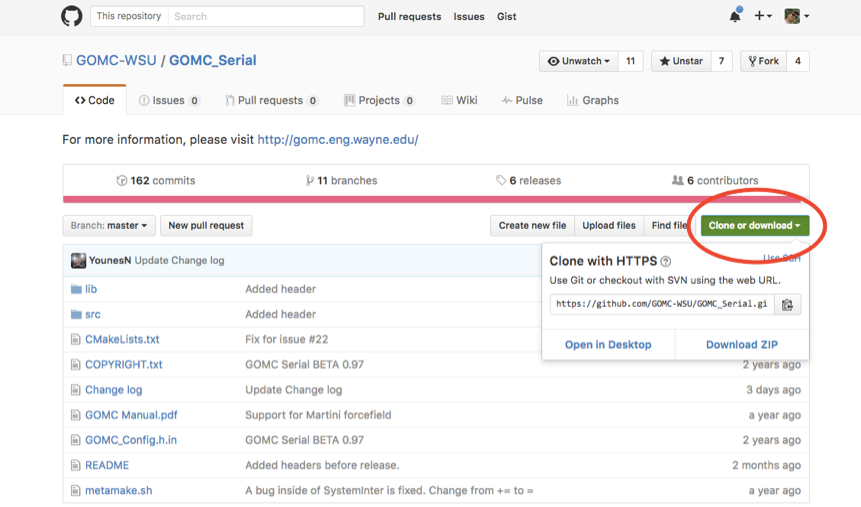
\includegraphics[scale=0.8]{images/clone}
\end{figure}

\section{Platform and Software Requirements}

\subsection{Supported Operating Systems}

GOMC officially supports Windows 7, 8, and most modern distributions of Linux (see the next section).  This software has the ability to compile on recent versions of OS X; however, such a platform is not officially supported. 

\subsection{Required Software Prequisites}

GOMC has some mild software requirements, which are widely available for Linux operating systems.  Required software requirements are:\\\\
\begin{easylist}[articletoc]
� C++03 Compliant Compiler
�� Linux/OS X
��� icc (Intel C++ Compiler)\\
Type the following command in a terminal: \\\\
\texttt{\$ icc --version} \\\\
If gives a version number 4.4 or later, you're all set.  If it's older than 4.4 (released in 2009), we recommend upgrading. \\
In Linux, the Intel compiler will generally produce the fastest serial executables (when running on Intel Core processors). \\\\
��� g++ (GNU GCC) \\
Type the following command in a terminal.\\\\
\texttt{\$ g++ --version}\\\\
If gives a version number 4.4 or later, you're all set. If it's older than 4.4 (released in 2009), we recommend upgrading.

�� Windows
��� Visual Studio\\
Microsoft's Visual Studio 2010 or later is recommended.\\
To check the version:\\
\textit{Help} (top tab) $\to$ \textit{About Microsoft Visual Studio}
\begin{figure}[H]
\centering
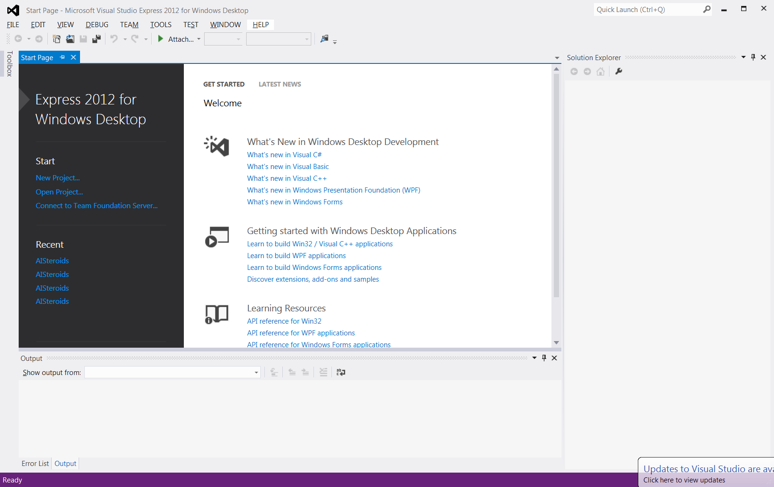
\includegraphics[scale=0.6]{images/vshelp}
\end{figure}
\begin{figure}[H]
\centering
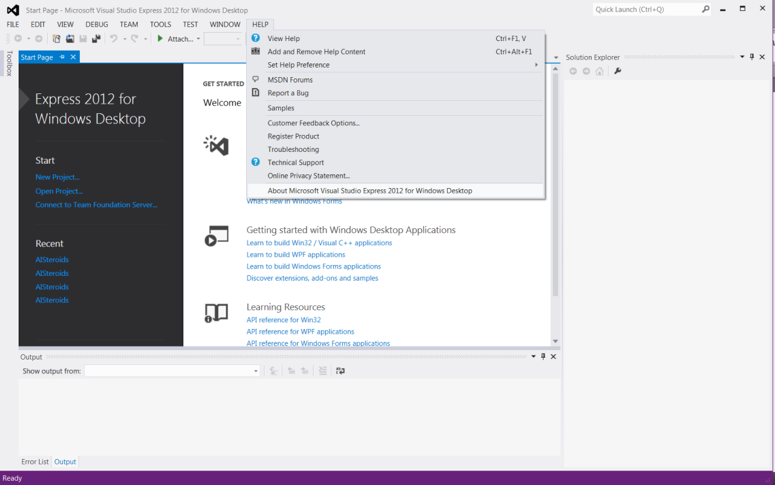
\includegraphics[scale=0.6]{images/vsabout}
\end{figure}

��� cmake (if compiling on Linux)\\
To check if cmake is installed:\\\\
\texttt{\$ which cmake}\\\\
To check the version number:\\\\
\texttt{\$ cmake --version}\\

��� nvcc/CUDA libs\\
The GPU builds of the code requires NVIDIA's CUDA 6.0 or newer:\\
To check if nvcc is installed:\\\\
\texttt{\$ which nvcc}\\\\
To check the version number:\\\\
\texttt{\$ nvcc --version}\\\\
CUDA is viewed as an essential requirement, but is not used to compile the serial code, which can be compiled on systems without CUDA.\\
To download CUDA visit NVIDIA's webpage:\\\\
\url{https://developer.nvidia.com/cuda-downloads}
\begin{figure}[H]
\centering
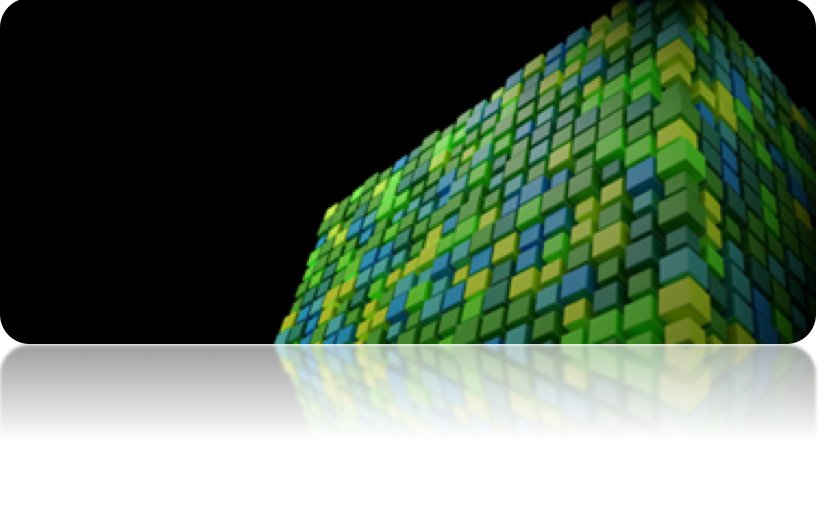
\includegraphics[scale=0.6]{images/cuda}
\end{figure}
CUDA is required to compile the GPU executable in both Windows and Linux.  Please refer to CUDA Developer webpages to select an appropriate version for the desired platform.\\
To install CUDA in Linux root/sudo, privileges are generally required.  In Windows, administrative access is required.
\end{easylist}

\section{Highly Recommended Software Tools}
\textit{\colorbox{yellow}{NOTE}: The listed programs are used in this manual and are generally considered necessary.}
\subsection{VMD}
VMD (Visual Molecular Dynamics) is a 3-D visualization and manipulation engine for molecular systems written in C-language. VMD is distributed and maintained by the University of Illinois at Urbana-Champaign.  Its sources and binaries are free to download. It comes with a robust scripting engine, which is capable of running python and tcl scripts.
More info can be found here:\\\\
\url{http://www.ks.uiuc.edu/Research/vmd/}\\\\
Although GOMC uses the same fundamental file types ? PDB (coordinates) and PSF (topology) as VMD, it uses some special tricks to obey certain rules of those file formats.\\
One useful purpose of VMD is visualization of your systems.
\begin{figure}[H]
\centering
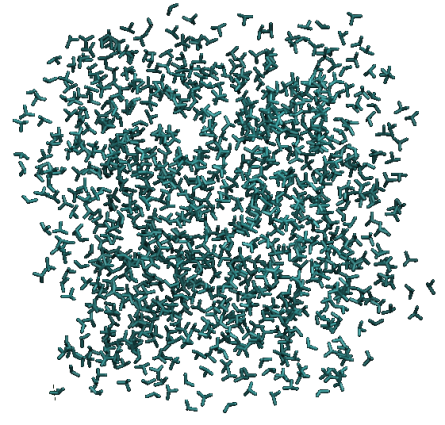
\includegraphics[scale=0.6]{images/vmd}
\caption{A system of united atom isobutane molecules}
\end{figure}
Nonetheless, the most critical part of VMD is a tool called PSFGen.  PSFGen uses a tcl or python script to generate a PDB and PSF file for a system of one or more molecules.  It is, perhaps, the most convenient way to generate a compliant PSF file.
\begin{figure}[H]
\centering
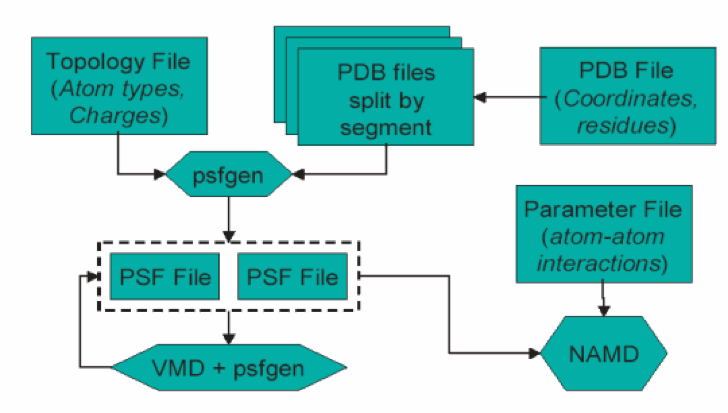
\includegraphics[scale=0.6]{images/psfgen}
\caption{An overview of the PSFGen file generation process and its relationship to VMD/NAMD}
\end{figure}
To read more about PSFGen, reference:\\\\
Plugin homepage @ UIUC\\
\url{http://www.ks.uiuc.edu/Research/vmd/plugins/psfgen}\\\\
``Generating a Protein Structure File (PSF)", part of the NAMD Tutorial from UIUC\\
\url{http://www.ks.uiuc.edu/Training/Tutorials/namd/namd-tutorial-html/node6.html}\\\\
In-Depth Overview [PDF]\\
\url{http://www.ks.uiuc.edu/Research/vmd/plugins/psfgen/ug.pdf}\\\\

\subsection{Packmol}
Packmol is a molecule packing tool created by Jos\'e Mario Mart\'inez, a professor of mathematics at the State University of Campinas, Brazil.  It is written in Fortran and is free to download.  More information is available on their homepage:\\\\
\url{http://www.ime.unicamp.br/~martinez/packmol}\\\\
To compile it, a Fortran language compiler is needed, such as gfortran.  Many Linux distributions no longer come with Fortran compilers automatically, so this may need to be installed additionally.\\
Packmol allows a specified number of molecules to be packed at defined separating distances within a certain region of space.  One of Packmol?s limitations is that it is unaware of topology; it treats each molecule or group of molecules as a rigid set of points.\\\\
\textit{\colorbox{red}{WARNING}: Another more serious limitation is that it is not aware of periodic boundary conditions (PBC).  As a result, when using Packmol to pack PDBs for GOMC, it is recommended to pack to a box 1 Angstroms smaller than the simulation box size.  This prevents hard overlaps over the periodic boundary.}

\section{Other Useful Software Tools}
\subsection{Grace}
Grace is a piece of graphing software written and maintained by the Weizmann Institute of Science's Plasma Laboratory (Rehovot, Israel). Mostly used in Linux, it can also be compiled in Windows.  The developers warn it may be missing some functionality.\\
\begin{figure}[H]
\centering

\includegraphics[scale=0.6]{images/grace}
\end{figure}
In-depth information and the source can be found on the project page, here:\\\\
\url{http://plasma-gate.weizmann.ac.il/Grace}\\\\
When compiled, Grace's executable in Linux is typically named ``xmgrace".  This tool allows the production of high quality, precise line and dot graphs, ideal for visualizing much of the thermodynamic data from the GOMC engine.  Below is an example of the results of simulations of saturated VLE densities of linear alkanes produced with Grace.
\begin{figure}[H]
\centering
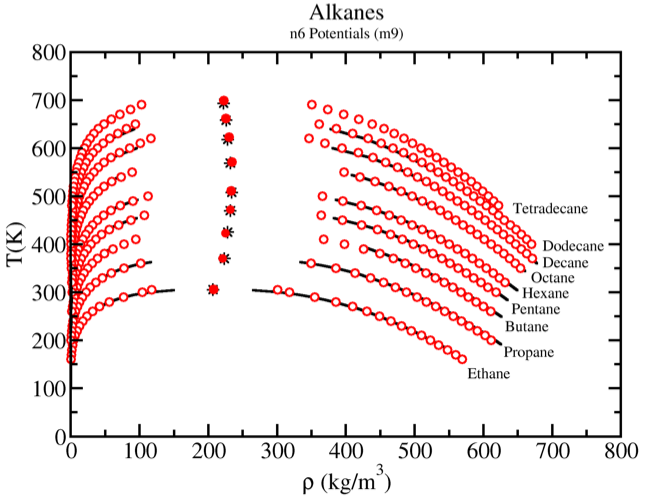
\includegraphics[scale=0.6]{images/alkanes}
\end{figure}

\subsection{Cygwin}
Cygwin is one option to assist in building and visualizing systems in Windows. It provides Microsoft Windows users with a Unix-like environment and command-line interface, and offers Windows-compatible ports of common Linux applications.\\\\
\url{https://cygwin.com}
\begin{figure}[H]
\centering
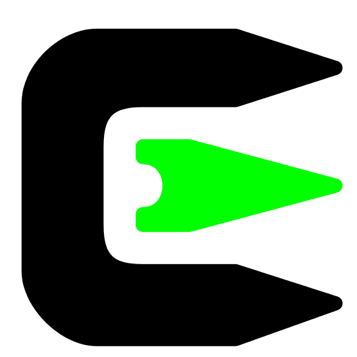
\includegraphics[scale=0.6]{images/cygwin}
\end{figure}
The software is a free and open source, licensed under the GNU General Public License version 3. Its primary maintainers are Red Hat Inc. and NetApp. One of the most impressive abilities of Cygwin is its ability to launch a full Windows-compatible X-server Window, which allows convenient visualization of Linux app GUIs. It is compatible with the Grace graphing software. In practice, this package behaves most analogously to a Linux virtual machine in Windows.

\section{Compiling GOMC}
\subsection{Extracting the code}
GOMC is distributed as a compressed folder, containing the source and build system. To compile the code after downloading it, the first step is to extract the compressed build folder.\\
In Windows, the folder for the GPU code is compressed using a standard *.zip file format. To unzip simply use a utility like Peazip: \\\\
\url{http://peazip.sourceforge.net/}\\\\
Below is an example of what the downloaded code looks like when unzipping in Peazip.
\begin{figure}[H]
\centering
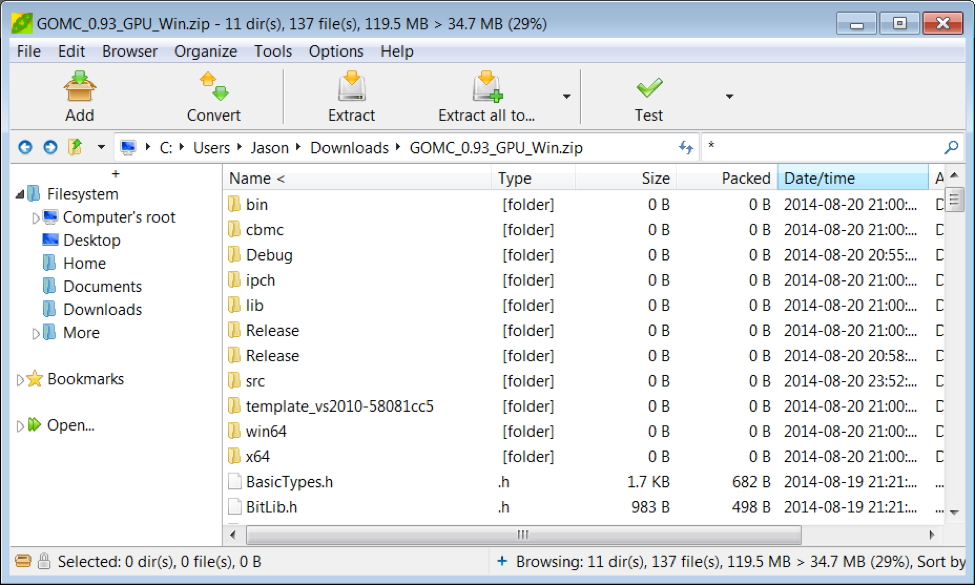
\includegraphics[scale=0.6]{images/peazip}
\end{figure}
In Linux, the GPU and Serial codes are compressed using gzip and tar (*.tar.gz).  To extract, simply move to the desire folder and type in the command line:\\\\
\texttt{\$ tar -xzvf <file name>.tar.gz}
\subsection{Compiling the code}
\subsubsection{GPU code}
\underline{Compilation on Windows}\\
Once the code is extracted, to compile it on Windows, you need to load the project into Visual Studio by opening the extracted folder and double clicking on the solution file of the desired Visual Studio version.  After the solution is opened in Visual Studio, go to the ``Build" menu and select ``Build solution" to compile the code. You can compile either with release mode or with debug mode by selecting the desired mode from the ``Solution Configuration" drop box. 
To run the project, simply click the run button or hit F5 on the keyboard.\\\\
\underline{Compilation on Linux}\\
To compile the GPU code on Linux, go to the directory of the project, and type in the command line:\\\\
\texttt{\$ make}\\\\
You can configure the ``makefile" file to choose different C compilers, to select the desired compute capability, and to configure many more compilation flags.\\
The default compute capability is 3.0. To change the compute capability, go to the \texttt{GENCODE\_FLAGS} option, and set it to one of the compute capability flags that are defined in the file.
\begin{minted}[frame=single,framesep=10pt]{make}
# CUDA code generation flags
GENCODE_SM10    := -gencode arch=compute_10,code=sm_10
GENCODE_SM10    := -gencode arch=compute_20,code=sm_20
GENCODE_SM10    := -gencode arch=compute_30,code=sm_30
GENCODE_SM10    := -gencode arch=compute_35,code=sm_35
GENCODE_FLAGS   := $(GENCODE_SM30)
\end{minted}
To run the program, run the executable ``GOMC.out".  The system's \texttt{LD\_LIBRARY\_PATH} will need to be configured to support CUDA (more on this later).
\subsubsection{Serial Code}
\underline{Compilation on Windows}\\
See GPU ``Compilation on Windows" section and follow an identical procedure for the released serial code. See \texttt{README} for instructions on how to use the CMake-GUI to build the configuration and solution files necessary for the Windows build.\\\\
\underline{Compilation on Linux}\\
In Linux, the CPU code uses a simple makefile. Enter the directory and type in the command line:\\\\
\texttt{\$ make all}\\\\
This will use the Makefile to compile a GPU-compatible executable called ``GOMC.out".  To run, the system?s \texttt{LD\_LIBRARY\_PATH} will need to be configured to support CUDA (more on this later).
For the serial code, which uses cmake for compilation, go to the base directory and type in the command line:\\\\
\texttt{\$ ./metamake.sh}\\\\
This cmake script will create a directory named ``bin".  Enter this directory:\\\\
\texttt{\$ cd bin}\\\\
and type:\\\\
\texttt{\$ make}\\\\
Four executables - \texttt{GOMC\_Serial\_GEMC} (Gibbs ensemble), \texttt{GOMC\_Serial\_NVT} (NVT ensemble), \texttt{GOMC\_Serial\_NPT} (isobaric-isothermal ensemble), and \texttt{GOMC\_Serial\_GCMC} (Grand canonical ensemble) - will be produced. By default, the distribution compiles in release mode.  To compile in debug mode (if you're using the code as a developer), open the file ``\texttt{CMakeCache.txt}" while still in the ``bin" folder.  This file contains information used by cmake to build the executables.  To compile in debug mode, change the value after ``\texttt{CMAKE\_BUILD\_TYPE:STRING=}" from ``Release" to ``Debug", and retype the command:\\\\ \texttt{\$ make}\\\\
The output executables should now be compiled with debugger symbols.
You can also swap the compiler by modifying the ``\texttt{CMAKE\_CXX\_COMPILER}" variable. For more information, refer to the CMake documentation.\\
Running GOMC in parallel using OpenMP:\\
To run the parallel version of CPU code, it needs to be compiled with openmp library. Open the file ``\texttt{CMakeCache.txt}", while still in the ``bin" folder, and change the value after ``\texttt{CMAKE\_CXX\_FLAGS\_RELEASE:STRING=}" from ``-O3 -DNDEBUG" to ``-O3 -qopenmp -DNDEBUG".\\
And retype the command:\\\\
\texttt{\$ make}\\\\
\section{Input File Formats}
In order to run simulation in GOMC, the following files need to be provided:
\begin{itemize}
\item GOMC executable
\item Input file ``NAME.conf" (proprietary control file)
\item PDB file(s)
\item PSF file(s)
\item Parameter file
\end{itemize}
\subsection{PDB File}
The PDB file stores coordinates for the simulation. The file format is widely adopted.
\begin{itemize}
\item Protein Databank (PDB) Files (plural: PDB files)
\item Open format, well-documented
\item Fixed-width format (hence white space is significant)
\item Up to 13.5m page views a month; up to 55.8m FTP requests per month
\item Used by NAMD, GROMACS, CHARMM, ACEMD, Amber
\end{itemize}
An overview of the PDB standard can be found here:\\\\
\url{http://www.wwpdb.org/docs.html}\\\\
The advantage of PDB files is their ubiquity and thorough documentation. Disadvantages include limited fixed point floating precision for coordinates, unused space, and proprietary implementations creating inconsistencies.\\
One PDB file is required per box. For NVT ensemble simulations, one file is expected; for Gibbs and grand canonical ensemble, two files are required.
GOMC recognizes the following keywords in PDB files:
\begin{itemize}
\item[$\diamondsuit$] \texttt{REMARK}
\item[$\diamondsuit$] \texttt{CRYST1}
\item[$\diamondsuit$] \texttt{ATOM}
\item[$\diamondsuit$] \texttt{END}
\end{itemize}
Currently, REMARK is ignored. Formerly, it was used to store proprietary information in frames (e.g. step number). Packmol typically leaves the following remark:\\\\
\begin{tabularx}{\textwidth}{| X | X | X | X | X | X |}
\hline
  \texttt{REMARK} & \texttt{original} & \texttt{generated} & \texttt{coordinate} & \texttt{pdb} & \texttt{file}  \\
\hline
\end{tabularx}\\\\
at the top of the file. Note that this is another example of an inconsistency with the spec. As of the PDB v3.30 specification the \texttt{REMARK} entry contains an identifying integer, which is supposed to occupy lines 8-10.\\
\begin{figure}[H]
\centering
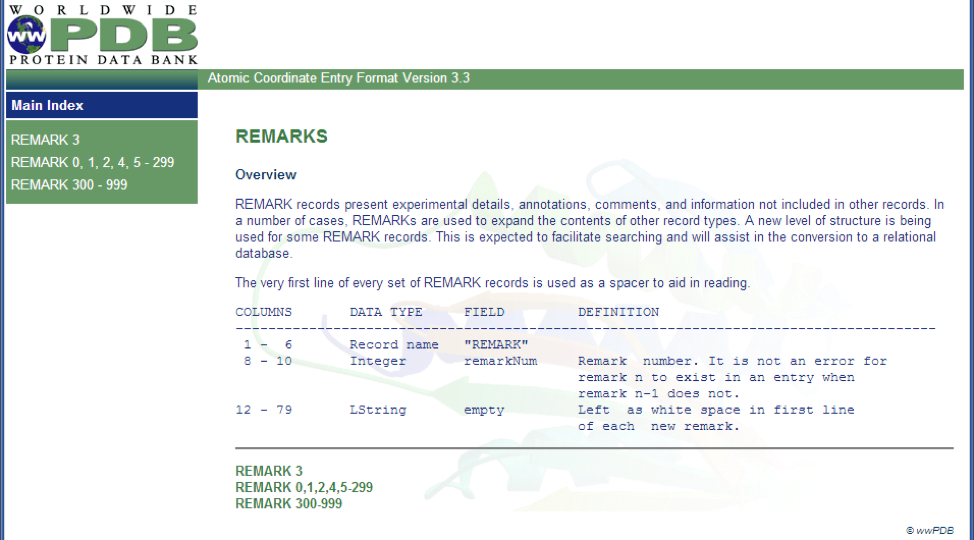
\includegraphics[scale=1.0]{images/remark}
\end{figure}
A file generated by Packmol has ``ori" in this position. Hence you may see future codes that are incompatible with this legacy kind of remarks.\\
Note also that the spaces 7 and 11 are not reserved; hence, they may be used in proprietary specifications.\\
\texttt{CRYST1} can be used to store the cell dimensions, which can also be put as a tag in the proprietary control file.\\
\url{http://www.wwpdb.org/documentation/format33/sect8.html#CRYST1}\\
\begin{figure}[H]
\centering
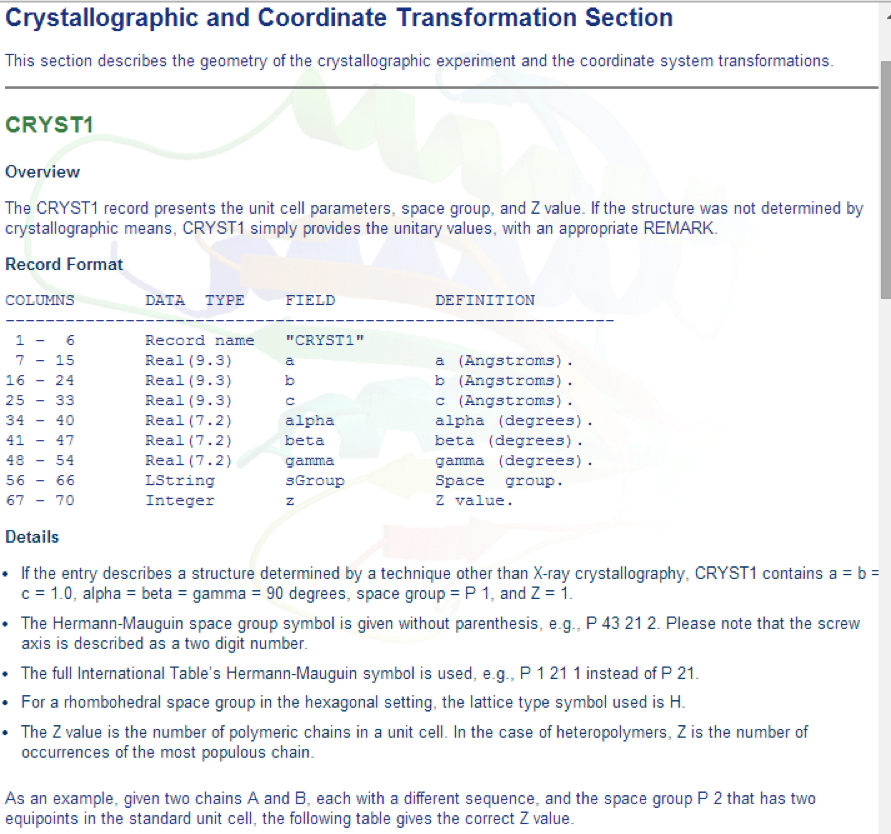
\includegraphics[scale=1.0]{images/pdb}
\end{figure}

%%%%% TODOOOOOOO 

\textit{\colorbox{yellow}{NOTE}: Only cubic and orthogonal cells are supported in this code.}
The main entry in the PDB file are \texttt{ATOM|} entries.  The keyword ``\texttt{ATOM}" is always followed by two spaces. An entry has a number of fields.
\begin{figure}[H]
\centering
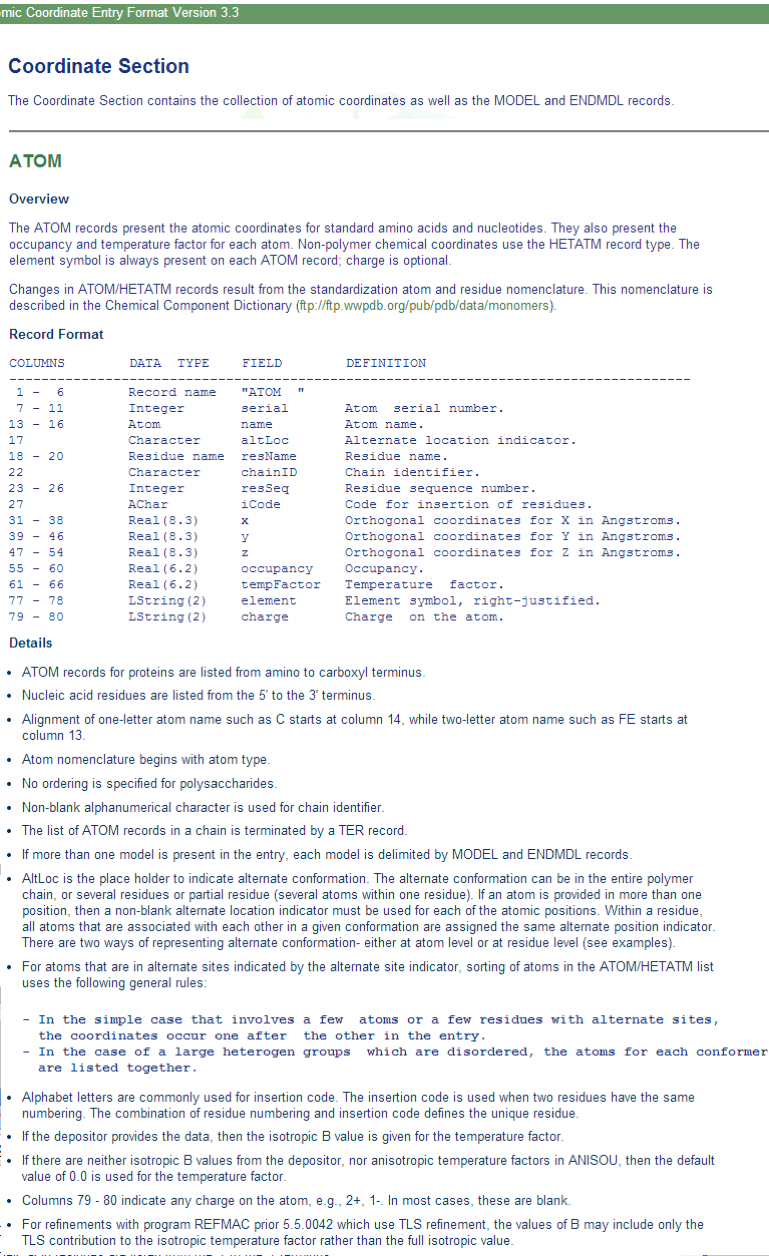
\includegraphics[scale=1.0]{images/atom}
\end{figure}
The key parameters are the coordinates x, y, and z. The precision is limited to eight whole decimal digits and three fractional decimal digits.\\
Other important entries are the residue name, atom name, and chain ID. Numbering is important primarily because it represents an inconvenience in packing/loading large systems. Revisiting the previous example,\\\\

%%%%% TODOOOOOOO

the atom name is ``C1" and residue name is ``ISB". The PSF file (next section) contains a lookup table of atoms. These contain the atom name from the PDB and the name of the atom kind in the parameter file it corresponds to. As multiple different atom names will all correspond to the same parameter, these can be viewed ``atom aliases" of sorts.  The chain letter (in this case `A') is sometimes used when packing a number of PDBs into a single PDB file.\\

A few important \colorbox{yellow}{Notes}/\colorbox{red}{Warnings} on Undocumented PDB Format Conventions:
\begin{itemize}
\item While it is explicitly stated in some other sections of the PDB file, the general convention observed by most codes is to right align when padding with white space.
\item Some codes (including PSFGen/VMD) use the 21st unused character to add a fourth letter to the residue (molecule name). This extension is currently supported, but is unofficial and, hence, may change in the future.
\item VMD requires a constant number of ATOMs in a multi-frame PDB (multiple records terminated by ``END" in a single file). To compensate for this, all atoms from all boxes in the system are written to the output PDBs of this code.
\item For atoms not currently in a box, the coordinates are set to $<0.00, 0.00, 0.00>$
\item The occupancy is commonly just set to ``1.00" and is left unused by many codes. We recycle this legacy parameter by using it to denote, in our output PDBs, the box a particle is in (box 0  occupancy=0.00 ; box 1  occupancy=1.00)
\item As the x, y, and z coordinates are fixed point with only three digits of precision, the energy values you get when restarting may be mildly different, particularly for bonded interactions due to roundoff in the coordinates.  This will eventually be remedied by the implementation of a full-precision trajectory (e.g. DCD) file.
\item The ``ISB" entry in columns 73-75 is not an official part of the PDB standard.  This is a proprietary entry called ``Segname", which has been embraced by NAMD and some other codes.
\end{itemize}
A frame in the PDB file is terminated with the keyword \texttt{END}.\\
With that overview of the format in mind, the following steps describe how a PDB file is typically built.\\
\begin{enumerate}
\item A single molecule PDB is obtained. In this example, the QM software package Gaussian was used to draw the molecule, which was then edited by hand to adhere to the PDB spec properly. The end result is a PDB for a single molecule:\\\\
\colorbox{lightgray}{
\begin{tabular}{*9l }
  \texttt{REMARK} & \multicolumn{8}{l}{\texttt{1 File created by GaussView 5.0.8}}  \\
  \texttt{ATOM} & \texttt{1} & \texttt{C1} & \texttt{ISB} & \texttt{1} & \texttt{0.911} & \texttt{-0.313} & \texttt{0.000} & \texttt{C} \\
  \texttt{ATOM} & \texttt{2} & \texttt{C2} & \texttt{ISB} & \texttt{1} & \texttt{1.424} & \texttt{-1.765} & \texttt{0.000} & \texttt{C} \\
  \texttt{ATOM} & \texttt{3} & \texttt{C3} & \texttt{ISB} & \texttt{1} & \texttt{-0.629} & \texttt{-0.313} & \texttt{0.000} & \texttt{C} \\
  \texttt{ATOM} & \texttt{4} & \texttt{C4} & \texttt{ISB} & \texttt{1} & \texttt{1.424} & \texttt{0.413} & \texttt{-1.257} & \texttt{C} \\
  \multicolumn{9}{l}{\texttt{END}} \\
\end{tabular}
}
\item Next, packings are calculated to place the simulation in a region of vapor-liquid coexistence. There are a couple of ways to do this in Gibbs ensemble:
\begin{itemize}
\item Pack both boxes to a single ?middle? density, which is an average of the liquid and vapor densities.
\item Same as 1, but add a modest amount to axis of one box (e.g. 10-30 A).  This technique can be handy in the constant pressure Gibbs ensemble.
\item Pack one box to the predicted liquid density and the other to the vapor density.
\end{itemize}
\begin{figure}[H]
\centering
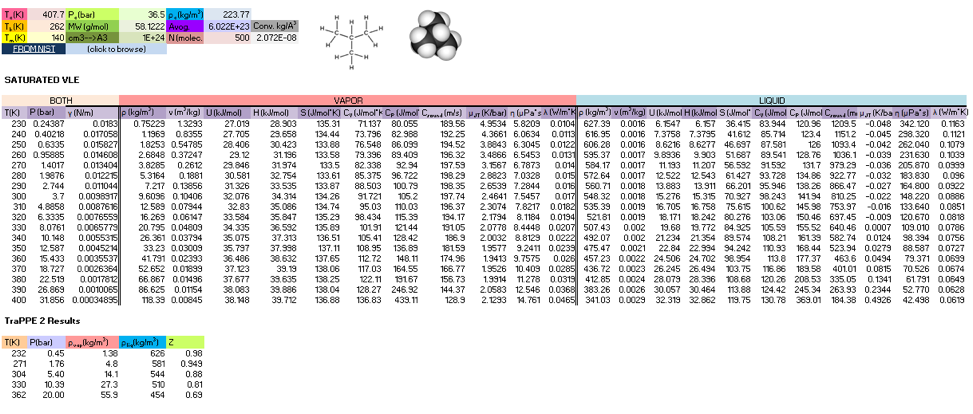
\includegraphics[scale=1.0]{images/pack2}
\end{figure}
A good reference for getting the information needed to estimate packing is the NIST Web Book database of pure compounds:\\\\
\url{http://webbook.nist.gov/chemistry/}\\\\
\item After packing is determined, a basic pack can be performed with a Packmol script.  Here is one example:\\\\
\colorbox{lightgray}{
\begin{tabular}{l}
\texttt{tolerance 3.0}\\
\texttt{filetype pdb}\\
\texttt{output STEP2\_ISB\_packed\_BOX\_0.pdb}\\\\
\texttt{structure isobutane.pdb}\\
\texttt{number 1000}\\
\texttt{inside box 0.1 0.1 0.1 70.20 70.20 70.20}\\
\texttt{end structure}
\end{tabular}
}\\\\
Packmol scripts are typically saved with the extension \texttt{*.inp}, so this might be named ``\texttt{pack\_isobutane.inp}".\\
To run the script, we type the following line into the terminal:\\\\
\texttt{\$ ./packmol < pack\_isobutane.inp}\\\\
\end{enumerate}
\subsection{PSF File}
The PSF file stores the topology, mass, charges, and atom identities of molecules in the system.
\begin{itemize}
\item Protein Structure File (PSF) 
\item Space-separated file
\item Used by NAMD, CHARMM, X-PLOR
\end{itemize}
The PSF file is not as robustly documented as the PDB format, but a basic description of it can be found here:\\\\
\url{http://www.ks.uiuc.edu/Training/Tutorials/namd/namd-tutorial-win-html/node24.html}\\\\
The PSF file is generally composed of a series of sections. A line with a numeric value is typically at the top of each section. This value lists the number of entries in that section (lines can contain multiple entries; a dihedral, for example has two quadruplet entries of atom indices per line). Note that outside the remarks and atom section, this number is typically smaller than the number of lines by a factor of 2 to 4.\\\\
PSF files always start with the string ``PSF" on their first line.\\\\
GOMC reuses PSF reading code from NAMD, hence it should have much of the same flexibility and limitations.  By section, the segments of a PSF file are:
\begin{itemize}
\item TITLE: remarks on the file
\item BONDS: the bonds (if applicable) in molecules 
\item ANGLE: the bonds (if applicable) in molecules
\item DIHEDRAL: the bonds (if applicable) in molecules
\item IMPROPER: the bonds (if applicable) in molecules
\item (other sections such as cross terms)
\end{itemize}
The code currently skips the title section and reads the bonds, angles, dihedrals and impropers.\\\\
A few important \colorbox{yellow}{Notes}/\colorbox{red}{Warnings}:
\begin{itemize}
\item The PSF file format is a highly redundant file format.  It repeats identical topology of thousands of molecules of a common kind in some cases. GOMC follows the same approach as NAMD, allowing this excess information externally and compiling it in the code.
\item Other sections (e.g. cross terms) contain unsupported or legacy parameters and are ignored.
\item Following the restrictions of VMD, the order of the PSF atoms must match the order in the PDB file.
\item Improper entries are read and stored, but are not currently used.  Support will eventually be added for this.
\end{itemize}
The PSF file is typically generated using PSFGen. It is convenient to make a script, such as the example below, to do this:\\\\
\colorbox{lightgray}{
\begin{tabular}{l}
\texttt{psfgen << ENDMOL}\\
\texttt{topology ./Top\_branched\_Alaknes.inp}\\
\texttt{segment ISB\{}\\
\texttt{    pdb ./STEP2\_ISB\_packed\_BOX\_0.pdb}\\
\texttt{    first none}\\
\texttt{    last none}\\
\texttt{\}}\\\\
\texttt{coordpdb ./STEP2\_ISB\_packed\_BOX\_0.pdb ISB}\\\\
\texttt{writepsf ./STEP3\_START\_ISB\_sys\_BOX\_0.psf}\\
\texttt{writepdb ./STEP3\_START\_ISB\_sys\_BOX\_0.pdb}\\
\end{tabular}
}\\\\
Typically, one script is run per box to generate a finalized PDB/PSF for that box. The script requires one additional file, the NAMD-style topology file. While GOMC does not directly read or interact with this file, it's typically used to generate the PSF and, hence, is considered one of the integral file types. It will be briefly discussed in the following section.\\\\

Here's a peek at how the generated PSF file looks for a packed isobutane system (abridged):\\\\
\colorbox{lightgray}{
\begin{tabular}{r l l l l l l l l}
\multicolumn{9}{l}{\texttt{PSF}}\\
\texttt{3} & \multicolumn{8}{l}{\texttt{!NTITLE}} \\
\texttt{REMARKS} & \multicolumn{8}{l}{\texttt{original generated structure x-plor psf file}}\\
\texttt{REMARKS} & \multicolumn{8}{l}{\texttt{topology ./Top\_Branched\_Alkanes.inp}}\\
\texttt{REMARKS} & \multicolumn{8}{l}{\texttt{segment ISB \{ first NONE; last NONE; auto angles dihedrals \}}}\\\\
\texttt{4000} & \multicolumn{8}{l}{\texttt{!NATOM}}\\
\texttt{1} & \texttt{ISB} & \texttt{1} & \texttt{ISB} & \texttt{C1} & \texttt{CH1} & \texttt{0.000000} & \texttt{13.0190} & \texttt{0}\\
\texttt{2} & \texttt{ISB} & \texttt{1} & \texttt{ISB} & \texttt{C2} & \texttt{CH3} & \texttt{0.000000} & \texttt{15.0350} & \texttt{0}\\
\texttt{3} & \texttt{ISB} & \texttt{1} & \texttt{ISB} & \texttt{C3} & \texttt{CH3} & \texttt{0.000000} & \texttt{15.0350} & \texttt{0}\\
\texttt{4} & \texttt{ISB} & \texttt{1} & \texttt{ISB} & \texttt{C4} & \texttt{CH3} & \texttt{0.000000} & \texttt{15.0350} & \texttt{0}\\
\texttt{5} & \texttt{ISB} & \texttt{2} & \texttt{ISB} & \texttt{C1} & \texttt{CH1} & \texttt{0.000000} & \texttt{13.0190} & \texttt{0}\\
\texttt{6} & \texttt{ISB} & \texttt{2} & \texttt{ISB} & \texttt{C2} & \texttt{CH3} & \texttt{0.000000} & \texttt{15.0350} & \texttt{0}\\
\texttt{7} & \texttt{ISB} & \texttt{2} & \texttt{ISB} & \texttt{C3} & \texttt{CH3} & \texttt{0.000000} & \texttt{15.0350} & \texttt{0}\\
\texttt{8} & \texttt{ISB} & \texttt{2} & \texttt{ISB} & \texttt{C4} & \texttt{CH3} & \texttt{0.000000} & \texttt{15.0350} & \texttt{0}\\
\multicolumn{9}{l}{\texttt{.}}\\
\multicolumn{9}{l}{\texttt{.}}\\
\multicolumn{9}{l}{\texttt{.}}\\
\texttt{3997} & \texttt{ISB} & \texttt{1000} & \texttt{ISB} & \texttt{C1} & \texttt{CH1} & \texttt{0.000000} & \texttt{13.0190} & \texttt{0}\\
\texttt{3998} & \texttt{ISB} & \texttt{1000} & \texttt{ISB} & \texttt{C2} & \texttt{CH3} & \texttt{0.000000} & \texttt{15.0350} & \texttt{0}\\
\texttt{3999} & \texttt{ISB} & \texttt{1000} & \texttt{ISB} & \texttt{C3} & \texttt{CH3} & \texttt{0.000000} & \texttt{15.0350} & \texttt{0}\\
\texttt{4000} & \texttt{ISB} & \texttt{1000} & \texttt{ISB} & \texttt{C4} & \texttt{CH3} & \texttt{0.000000} & \texttt{15.0350} & \texttt{0}\\
\texttt{3000} & \texttt{!BOND:} & \multicolumn{7}{l}{bonds}\\
\texttt{1} & \texttt{2} & \texttt{1} & \texttt{3} & \texttt{1} & \texttt{4} & \texttt{5} & \multicolumn{2}{l}{\texttt{6}}\\ 
\texttt{5} & \texttt{7} & \texttt{5} & \multicolumn{2}{l}{\texttt{8}}\\ 
\multicolumn{9}{l}{\texttt{.}}\\
\multicolumn{9}{l}{\texttt{.}}\\
\multicolumn{9}{l}{\texttt{.}}\\
\texttt{3997} & \texttt{3998} & \texttt{3997} & \texttt{3998} & \texttt{3999} & \texttt{3997} & \multicolumn{3}{l}{\texttt{4000}}\\
\texttt{3000} & \texttt{!NTHETA:} & \multicolumn{7}{l}{\texttt{angles}}\\
\texttt{2} & \texttt{1} & \texttt{4} & \texttt{2} & \texttt{1} & \texttt{3} & \texttt{3} & \texttt{1} & \texttt{4}\\
\texttt{6} & \texttt{5} & \texttt{8} & \texttt{6} & \texttt{5} & \texttt{7} & \texttt{7} & \texttt{5} & \texttt{8}\\
\multicolumn{9}{l}{\texttt{.}}\\
\multicolumn{9}{l}{\texttt{.}}\\
\multicolumn{9}{l}{\texttt{.}}\\
\texttt{3998} & \texttt{3997} & \texttt{4000} & \texttt{3998} & \texttt{3997} & \texttt{3999} & \texttt{3999} & \texttt{3997} & \texttt{4000}\\\\
\texttt{0} & \multicolumn{8}{l}{\texttt{!NPHI: dihedrals}}\\
\texttt{0} & \multicolumn{8}{l}{\texttt{!NIMPHI: impropers}}\\
\texttt{0} & \multicolumn{8}{l}{\texttt{!NDON: donors}}\\
\texttt{0} & \multicolumn{8}{l}{\texttt{!NACC: acceptors}}\\
\texttt{0} & \multicolumn{8}{l}{\texttt{!NNB}}\\
\texttt{0} & \texttt{0} & \texttt{0} & \texttt{0} & \texttt{0} & \texttt{0} & \texttt{0} & \multicolumn{2}{l}{\texttt{0}}\\
\texttt{0} & \texttt{0} & \texttt{0} & \texttt{0} & \texttt{0} & \texttt{0} & \texttt{0} & \multicolumn{2}{l}{\texttt{0}}\\
\multicolumn{9}{l}{\texttt{.}}\\
\multicolumn{9}{l}{\texttt{.}}\\
\multicolumn{9}{l}{\texttt{.}}\\
\end{tabular}
}\\\\
\subsection{Topology File}
The topology is a whitespace separated file format, which contains a list of atoms and  their corresponding masses, and a list of residue information (charges, composition, and topology). Essentially, it is a non-redundant lookup table equivalent to the PSF file.\\\\
This is followed by a series of residues, which tell PSFGen what atoms are bonded to a given atom. Each residue is comprised of four key elements:
\begin{itemize}
\item A header beginning with the keyword RESI with the residue name and net charge
\item A body with multiple ATOM entries (not to be confused with the PDB-style entries of the same name), which list the partial charge on the particle and what kind of atom each named atom in a specific molecule/residue is.
\item A section of lines starting with the word BOND contains pairs of bonded atoms (typically 3 per line)
\item A closing section with instructions for PSFGen.
\end{itemize}
Here's an example of a residue definition for isobutane:\\\\
\colorbox{lightgray}{
\begin{tabular}{l}
\texttt{RESI ISB ~~ 0.00 ! isobutane - TraPPE}\\
\texttt{GROUP}\\
\texttt{ATOM C1 CH1    0.00 !    C3}\\
\texttt{ATOM C2 CH3    0.00 ! C2-C1}\\
\texttt{ATOM C3 CH3    0.00 !    C4}\\
\texttt{ATOM C4 CH3    0.00 !}\\
\texttt{BOND C1 C2 C1 C3 C1 C4}\\
\texttt{PATCHING FIRS NONE LAST NONE}
\end{tabular}}\\\\
Here's a full parameter file prepared to pack a system of isobutane:\\\\
\colorbox{lightgray}{
\begin{tabular}{l}
\texttt{*}\\
\texttt{* Custom top file -- branched alkanes}\\
\texttt{*}\\
\texttt{1  1}\\
\texttt{!}\\
\texttt{MASS   1  CH3  15.035 C !}\\
\texttt{MASS   2  CH1  13.019 C !}\\\\
\texttt{RESI ISB ~~ 0.00 ! isobutane - TraPPE}\\
\texttt{GROUP}\\
\texttt{ATOM C1 CH1    0.00 !    C3}\\
\texttt{ATOM C2 CH3    0.00 ! C2-C1}\\
\texttt{ATOM C3 CH3    0.00 !    C4}\\
\texttt{ATOM C4 CH3    0.00 !}\\
\texttt{BOND C1 C2 C1 C3 C1 C4}\\
\texttt{PATCHING FIRS NONE LAST NONE}\\\\
\texttt{END}
\end{tabular}}\\\\
Note that the keyword \texttt{END} must be used to terminate this file and keywords related to the auto-generation process must be placed near the top of the file, after the MASS definitions.\\\\
More in-depth information can be found in the following links:\\
``Topology Tutorial" (PDF, in-depth)\\
\url{http://www.ks.uiuc.edu/Training/Tutorials/science/topology/topology-tutorial.pdf}\\
``NAMD Tutorial: 4. Examining the Topology File"\\
\url{http://www.ks.uiuc.edu/Training/Tutorials/science/topology/topology-html/node4.html}\\
``Developing Topology and Parameter Files"\\
\url{http://www.ks.uiuc.edu/Training/Tutorials/science/force field-tutorial/force field-html/node6.html}\\
``NAMD Tutorial: 25. Topology Files"\\
\url{http://www.ks.uiuc.edu/Training/Tutorials/namd/namd-tutorial-win-html/node25.html}

\colorbox{yellow}{\texttt{NOTE:}} Links are courtesy of UIUC.\\
\subsection{Parameter File(s):}
Currently, GOMC uses a single parameter file and the user has the two kinds of parameter file choices:
\begin{itemize}
\item ``\texttt{CHARMM}" (Chemistry at Harvard Molecular Mechanics) compatible parameter file
\item ``\texttt{EXOTIC}" parameter file
\end{itemize}
If the parameter file type is not specified or if the chosen file is missing, an error will result.\\
Both force field file options are whitespace separated files with sections preceded by a tag. When a known tag (representing a molecular interaction in the model) is encountered, reading of that section of the force field begins.  Comments (anything after a * or !) and whitespace are ignored. Reading concludes when the end of the file is reached or another section tag is encountered.\\\\
\underline{CHARMM format parameter file}\\
\texttt{CHARMM} contains a widely used model for describing energies in Monte Carlo and molecular dynamics simulations. It is intended to be compatible with other codes that use such a format, such as \texttt{NAMD}.
For a general overview of the \texttt{CHARMM} force field, see:\\
\url{http://www.charmmtutorial.org/index.php/The_Energy_Function}\\\\
Here's the basic \texttt{CHARMM} contributions that are supported in GOMC:

\begin{align*}
U_{\texttt{bond}}&=\sum_{\texttt{bonds}} K_b(b-b_0)^2 & U_{\texttt{dihedral}}&=\sum_{\texttt{dihedrals}} K_{\phi} [1+\cos(n\phi - \delta)]\\
U_{\texttt{angle}}&=\sum_{\texttt{angles}} K_{\theta}(\theta-\theta_0)^2 & U_{\texttt{LJ}} &=\sum_{\texttt{nonbonded}} \epsilon_{ij}\left[\left(\frac{R_{min_{ij}}}{r_{ij}}\right)^{12}-2\left(\frac{R_{min_{ij}}}{r_{ij}}\right)^6\right]+ \frac{q_i q_j}{\epsilon r_{ij}} \\
\end{align*}

As seen above, the following are recognized, read and used:
\begin{itemize}
\item \texttt{BONDS}
\begin{itemize}
\item Quadratic expression describing bond stretching based on bond length (b) in Angstrom
\item Typically, it is ignored as bonds are rigid for Monte Carlo simulations. To specify that it is to be ignored, put a very large value i.e. ``999999999999" for $K_b$.
\end{itemize}
\colorbox{yellow}{\texttt{NOTE:}} GOMC does not sample bond stretch.
\begin{figure}[H]
\centering
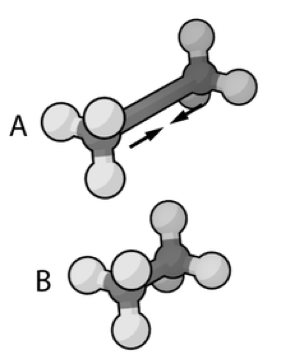
\includegraphics[scale=1.0]{images/bonds}
\caption{Image Courtesy of Wikimedia Commons}
\end{figure}
\item \texttt{ANGLES}
\begin{itemize}
\item Describe the conformational lbehavior of an angle ($\vartheta$) between three atoms, one of which is shared branch point to the other two. To fix any angle and ignore the related angle energy, put a very large value i.e. ``999999999999" for $K_{\theta}$.
\begin{figure}[H]
\centering
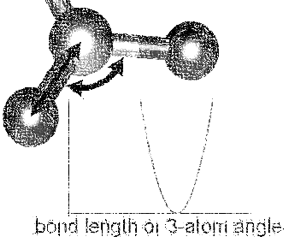
\includegraphics[scale=1.0]{images/angle}
\caption{Image Courtesy of Wikimedia Commons}
\end{figure}
\end{itemize}
\item \texttt{DIHEDRALS} 
\begin{itemize}
\item Describes crankshaft-like rotation behavior about a central bond in a series of three consecutive bonds (rotation is given as $\phi$).
\end{itemize}
\begin{figure}[H]
\centering
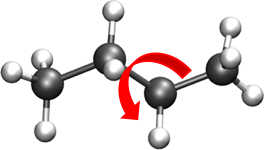
\includegraphics[scale=1.0]{images/dihedrals}
\caption{Image Courtesy of Wikimedia Commons}
\end{figure}
\item \texttt{NONBONDED}
\begin{itemize}
\item This tag name only should be used if \texttt{CHARMM} force files are being used. This section describes 12-6 (Lennard-Jones) non-bonded interactions. Non-bonded parameters are assigned by specifying atom type name followed by polarizabilities (which will be ignored), minimum energy, and (minimum radius)/2. In order to modify 1-4 interaction, a second polarizability (again, will be ignored), minimum energy, and (minimum radius)/2 need to be defined; otherwise, the same parameter will be considered for 1-4 interaction.
\end{itemize}
\begin{figure}[H]
\centering
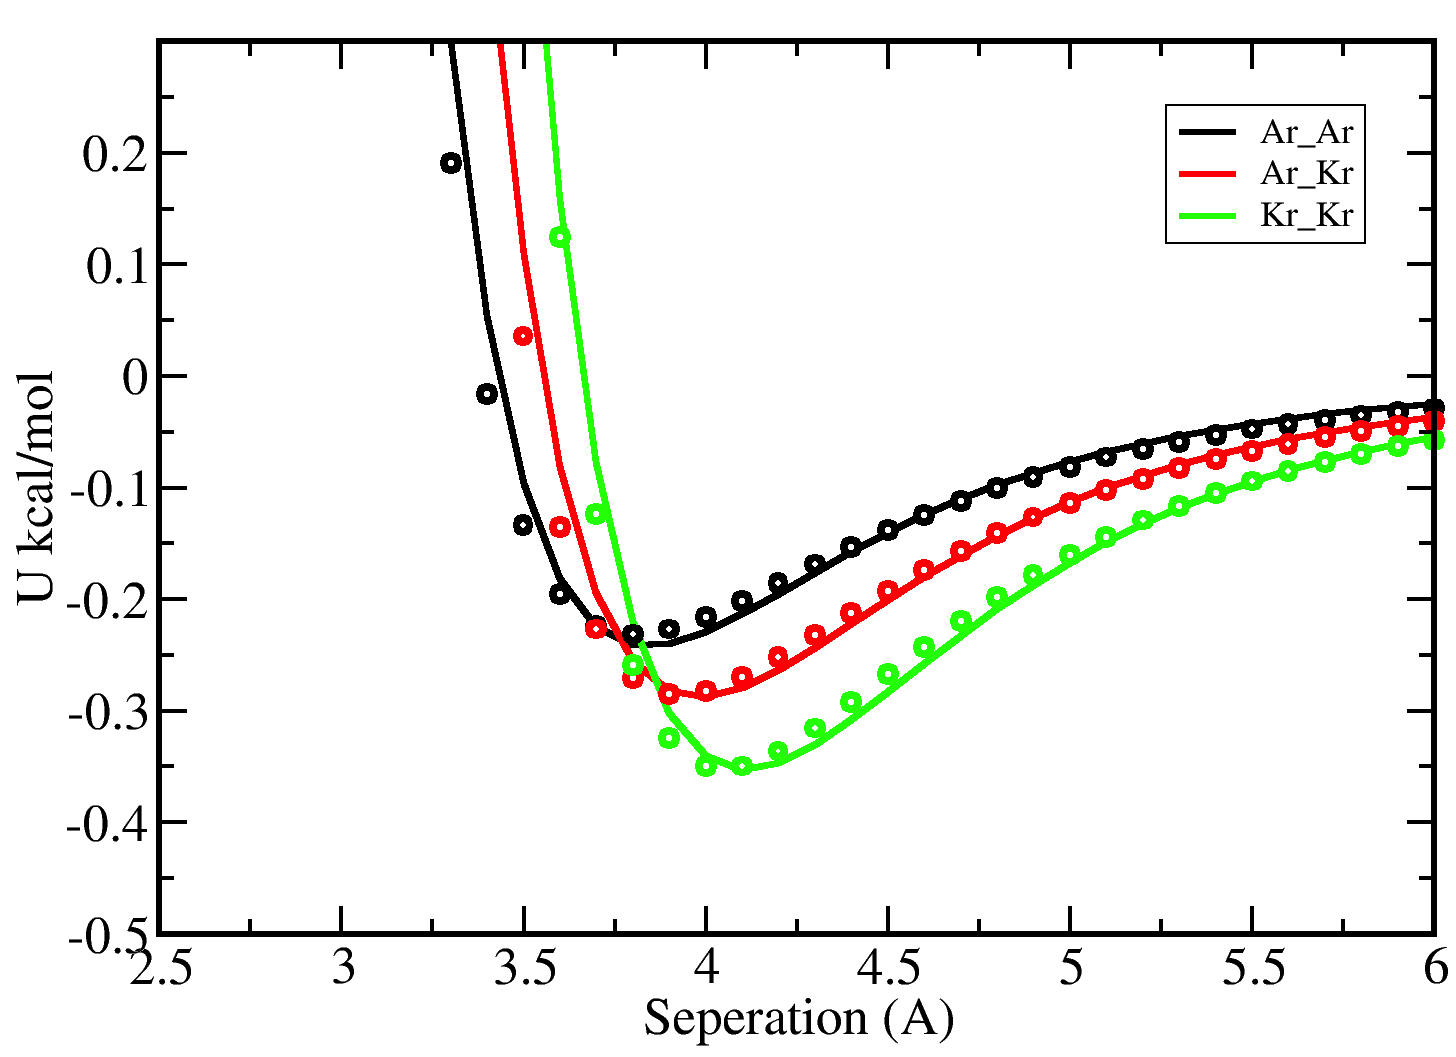
\includegraphics[scale=1.0]{images/nonbonded}
\caption{Image Courtesy of Wikimedia Commons}
\end{figure}

\item \texttt{NBFIX}
\begin{itemize}
\item This tag name only should be used if \texttt{CHARMM} force field is being used. This section allows interaction between two pairs of atoms to be modified, done by specifying two atom type names followed by minimum energy and minimum radius. In order to modify 1-4 interaction, a second minimum energy and minimum radius need to be defined; otherwise, the same parameter will be considered for 1-4 interaction.\\
\colorbox{yellow}{\texttt{NOTE:}} Please pay attention that in this section we define minimum radius, not (minimum radius)/2 as it is defined in the \texttt{NONBONDED} section.
\end{itemize}
Currently, supported sections of the \texttt{CHARMM} compliant file include \texttt{BONDS}, \texttt{ANGLES}, \texttt{DIHEDRALS}, \texttt{NONBONDED}, \texttt{NBFIX}. Other sections such as \texttt{CMAP} are not currently read or supported.\\
\end{itemize}
\subsubsection{BONDS}
(``bond stretching") is one key section of the \texttt{CHARMM}-compliant file. Units for the \texttt{$K_b$} variable in this section are in kcal/mol; the \texttt{$b_0$} section (which represents the equilibrium bond length for that kind of pair) is measured in Angstroms.\\\\
\colorbox{lightgray}{
\begin{tabular}{l}
\texttt{BONDS}\\
\texttt{!V(bond) = Kb(b - b0)**2}\\
\texttt{!}\\
\texttt{!Kb: kcal/mole/A**2}\\
\texttt{!b0: A}\\
\texttt{!}\\
\texttt{! Kb (kcal/mol) = Kb (K) * Boltz. const.; }\\
\texttt{!}\\
\texttt{!atom type     Kb              b0        description}\\
\texttt{CH3 CH1        9999999999      1.540   ! TraPPE 2}\\
\end{tabular}}\\\\
\colorbox{yellow}{\texttt{NOTE:}} The \texttt{$K_b$} value may appear odd, but this is because a larger value corresponds to a more rigid bond. As Monte Carlo force fields (e.g. \texttt{TraPPE}) typically treat molecules as rigid constructs, \texttt{$K_b$} is set to a large value - 9999999999. Sampling bond stretch is not supported in GOMC.\\\\
\subsubsection{ANGLES}
(``bond bending"), where \texttt{$\theta$} and \texttt{$\theta_0$} are commonly measured in degrees and \texttt{$K_{\theta}$} is measured in kcal/mol/K.  These values, in literature, are often expressed in Kelvin (K). To convert Kelvin to kcal/mol/K, multiply by the Boltzmann constant -- \texttt{$K_b$} , 0.0019872041 kcal/mol. In order to fix the angle, it requires to set a large value for \texttt{$K_{\theta}$}. By assigning a large value like 9999999999, specified angle will be fixed and energy of that angle will considered to be zero.\\\\
Here is an example of what is necessary for isobutane:\\
\colorbox{lightgray}{
\begin{tabular}{l}
\texttt{ANGLES}\\
\texttt{!}\\
\texttt{!V(angle) = Ktheta(Theta - Theta0)**2}\\
\texttt{!}\\
\texttt{!V(Urey-Bradley) = Kub(S - S0)**2}\\
\texttt{!}\\
\texttt{!Ktheta: kcal/mole/rad**2}\\
\texttt{!Theta0: degrees}\\
\texttt{!S0: A}\\
\texttt{!}\\
\texttt{! Ktheta (kcal/mol) = Ktheta (K) * Boltz. const.}\\
\texttt{!}\\
\texttt{!atom types         Ktheta       Theta0   Kub(?)  S0(?)}\\
\texttt{CH3 CH1 CH3         62.100125    112.00 ! TraPPE 2}\\
\end{tabular}}\\\\
Some CHARMM \texttt{ANGLES} section entries include Urey-Bradley potentials (\texttt{$K_{ub}$}, \texttt{$b_{ub}$}), in addition to the standard quadratic angle potential. The constants related to this potential function are currently read, but the logic has not been added to calculate this potential function. Support for this potential function will be added in later versions of the code.\\\\
The final major bonded interactions section of the \texttt{CHARMM} compliant parameter file are the \texttt{DIHEDRALS}. Each dihedral is composed of a dihedral series of 1 or more terms. Often, there are 4 to 6 terms in a dihedral. Angles for the dihedrals' deltas are given in degrees.\\
Since isobutane has no dihedral, here are the parameters pertaining to 2,3-dimethylbutane:\\\\
\colorbox{lightgray}{
\begin{tabular}{l}
\texttt{DIHEDRALS}\\
\texttt{!}\\
\texttt{!V(dihedral) = Kchi(1 + cos(n(chi) - delta))}\\
\texttt{!}\\
\texttt{!Kchi: kcal/mole}\\
\texttt{!n: multiplicity}\\
\texttt{!delta: degrees}\\
\texttt{!}\\
\texttt{! Kchi (kcal/mol) = Kchi (K) * Boltz. const.}\\
\texttt{!}\\
\texttt{!atom types         Kchi        n    delta              description}\\
\texttt{X   CH1 CH1 X      -0.498907    0      0.0              ! TraPPE 2}\\
\texttt{X   CH1 CH1 X       0.851974    1      0.0              ! TraPPE 2}\\
\texttt{X   CH1 CH1 X      -0.222269    2    180.0              ! TraPPE 2}\\
\texttt{X   CH1 CH1 X       0.876894    3      0.0              ! TraPPE 2}\\
\end{tabular}}\\\\
\colorbox{yellow}{\texttt{NOTE:}} The code allows the use of `X' to indicate ambiguous positions on the ends. This is useful because this kind is often determined solely by the two middle atoms in the middle of the dihedral, according to literature.
\subsubsection{IMPROPERS}
Energy parameters used to describe out-of-plane rocking are currently read, but unused. The section is often blank. If it becomes necessary, algorithms to calculate the improper energy will need to be added.\\
The next section of the \texttt{CHARMM} style parameter file is the \texttt{NONBONDED}. In order to use \texttt{TraPPE} this section of the \texttt{CHARMM} compliant file is critical. Here's an example with our isobutane potential model:\\\\
\colorbox{lightgray}{
\begin{tabular}{l}
\texttt{NONBONDED }\\
\texttt{!}\\
\texttt{!V(Lennard-Jones) = Eps,i,j[(Rmin,i,j/ri,j)**12 - 2(Rmin,i,j/ri,j)**6]}\\
\texttt{!}\\
\texttt{!atom  ignored   epsilon     Rmin/2       ignored  eps,1-4  Rmin/2,1-4}\\
\texttt{!}\\
\texttt{CH3    0.0      -0.194745992  2.10461634058 0.0   0.0   0.0 ! TraPPE 1}\\
\texttt{CH1    0.0      -0.019872040  2.62656119304 0.0   0.0   0.0! TraPPE 2}\\
\texttt{End}\\
\end{tabular}}\\\\
\colorbox{yellow}{\texttt{NOTE:}} The \texttt{$R_{min}$} is different from \texttt{$\sigma$}. \texttt{$\sigma$} is the distance to the x-intercept (where interaction energy goes from being repulsive to positive). \texttt{$R_{min}$} is the potential well-depth, where the attraction is maximum. To convert \texttt{$\sigma$} to \texttt{$R_{min}$}, simply multiply \texttt{$\sigma$} by 0.56123102415, and flag it with a negative sign.\\
The last section of the \texttt{CHARMM} style parameter file is the \texttt{NBFIX}. In this section, individual pair interaction will be modified. First, pseudo non-bonded parameters have to be defined in \texttt{NONBONDED} and modified in \texttt{NBFIX}. Here?s an example if it is required to modify interaction between \texttt{CH3} and \texttt{CH1} atoms:\\
\colorbox{lightgray}{
\begin{tabular}{l}
\texttt{NBFIX }\\
\texttt{!V(Lennard-Jones) = Eps,i,j[(Rmin,i,j/ri,j)**12 - 2(Rmin,i,j/ri,j)**6]}\\
\texttt{!}\\
\texttt{!atom  atom  epsilon      Rmin  eps,1-4  Rmin,1-4}\\
\texttt{CH3   CH1    -0.294745992 1.10461634058 ! }\\
\texttt{End}\\
\end{tabular}}\\\\

\subsection{Exotic Parameter file}
The exotic file is intended for use with nonstandard/specialty models of molecular interaction, which are not included in \texttt{CHARMM} standard. Currently, two custom interaction are included:
\begin{description}
\item [NONBODED\_MIE] This section describes n-6 (Lennard-Jones) non-bonded interactions. The Lennard-Jones potential (12-6) is a subset of this potential. Non-bonded parameters are assigned by specifying atom type name followed by minimum energy, atom diameter, and repulsion exponent. In order to modify 1-4 interaction, a second minimum energy, atom diameter, and repulsion exponent need to be defined; otherwise, the same parameters would be considered for 1-4 interaction.
\item [NBFIX\_MIE] This section allows n-6 (Lennard-Jones) interaction between two pairs of atoms to be modified. This is done by specifying two atoms type names followed by minimum energy, atom diameter, and repulsion exponent. In order to modify 1-4 interaction, a second minimum energy, atom diameter, and repulsion exponent need to be defined; otherwise, the same parameter will be considered for 1-4 interaction.
\end{description}
\colorbox{yellow}{\texttt{NOTE:}} In \texttt{EXOTIC} force field, the definition of atom diameter($\sigma$) is same for both \texttt{NONBONDED\_MIE} and \texttt{NBFIX\_MIE}.\\
Otherwise, the exotic file reuses the same geometry section headings - \texttt{BONDS} / \texttt{ANGLES} / \texttt{DIHEDRALS} / etc. The only difference in these sections versus in the \texttt{CHARMM} format force field file is that the energies are in Kelvin (`K'), the unit most commonly found for parameters in Monte Carlo chemical simulation literature. This precludes the need to convert to kcal/mol, the energy unit used in \texttt{CHARMM}.\\
The most frequently used section of the exotic files in the Mie potential section is \texttt{NONBONDED\_MIE}.\\
Here are the parameters that are used to simulate alkanes:\\\\
\colorbox{lightgray}{
\begin{tabular}{l}
\texttt{NONBONDED\_MIE}\\
\texttt{!}\\
\texttt{!V(mie) = 4*eps*((sig\_ij/r\_ij)\^n-(sig\_ij/r\_ij)\^6)}\\
\texttt{!}\\
\texttt{!atom   eps          sig        n    eps,1-4    sig,1-4     n,1-4 }\\
\texttt{CH4     161.00       3.740      14   0.0 0.0 0.0 ! Potoff, et al. '09}\\
\texttt{CH3     121.25       3.783      16   0.0 0.0 0.0 ! Potoff, et al. '09}\\
\texttt{CH2      61.00       3.990      16   0.0 0.0 0.0 ! Potoff, et al. '09}\\
\end{tabular}}\\\\
\colorbox{yellow}{\texttt{NOTE:}} Although the units (Angstroms) are the same, the exotic file uses $\sigma$, not the $R_{min}$ used by \texttt{CHARMM}. The energy in the exotic file are expressed in Kelvin (K), as this is the standard convention in the literature.\\
\subsection{Control File (*.conf)}
The control file is GOMC's proprietary input file. It contains key settings. The settings generally fall under three categories:
\begin{itemize}
\item Input/Simulation Setup
\item System Settings for During Run
\item Output Settings
\end{itemize}
\colorbox{yellow}{\texttt{NOTE:}} The control file is designed to recognize logic values, such as ``yes/true/on" or ``no/false/off".\\
\subsubsection{Input/Simulation Setup}
In this section, input file names are listed. In addition, if you want to restart your simulation or use integer seed for running your simulation, you need to modify this section according to your purpose.
\begin{description}
\item [Restart] Determines whether to restart and, if so, what step to restart from.\\
	\begin{itemize}
	\item Value 1: $<BOOLEAN>$ - true if restart, false otherwise\\
	\end{itemize}
\item [FirstStep] Determines what step to restart from. If Restart was set to true, step number needs to be specified; otherwise, the program will terminate.\\
	\begin{itemize}
	\item Value 1: $<ULONG>$ - step to restart from\\
	\colorbox{lightgray}{
	\begin{tabular}{l}
	\texttt{\#\#\#\#\#\#\#\#\#\#\#\#\#\#\#\#\#\#\#\#\#\#\#\#\#\#\#\#\#\#\#\#\#}\\
	\texttt{\# enable, step}\\
	\texttt{\#\#\#\#\#\#\#\#\#\#\#\#\#\#\#\#\#\#\#\#\#\#\#\#\#\#\#\#\#\#\#\#\#}\\
	\texttt{Restart     true}\\
	\texttt{FirstStep   1000000}\\
	\end{tabular}}
	\end{itemize}
\item [PRNG] Dictates how to start the pseudo-random number generator (PRNG)
	\begin{itemize}
	\item Value 1: $<STRING>$
		\begin{itemize}
		\item \texttt{RANDOM}: Randomizes Mersenne Twister PRNG with random bits based on the system time.
		\colorbox{lightgray}{
		\begin{tabular}{l}
		\texttt{\#\#\#\#\#\#\#\#\#\#\#\#\#\#\#\#\#\#\#\#\#\#\#\#\#\#\#\#\#\#\#\#\#}\\
		\texttt{\# kind \{RESTART, RANDOM, INTSEED\}}\\
		\texttt{\#\#\#\#\#\#\#\#\#\#\#\#\#\#\#\#\#\#\#\#\#\#\#\#\#\#\#\#\#\#\#\#\#}\\
		\texttt{PRNG RANDOM}\\
		\end{tabular}}
		\item \texttt{INTSEED}: This option ``seeds" the Mersenne Twister PRNG with a standard integer. When the same integer is used, the generated PRNG stream should be the same every time, which is helpful in tracking down bugs.
		\item \texttt{RESTART}: Used for restarting a previous simulation. This option in the Mersenne Twister's state from a saved file.\\
		\colorbox{lightgray}{
		\begin{tabular}{l}
		\texttt{\#\#\#\#\#\#\#\#\#\#\#\#\#\#\#\#\#\#\#\#\#\#\#\#\#\#\#\#\#\#\#\#\#}\\
		\texttt{\# kind \{RESTART, RANDOM, INTSEED\}}\\
		\texttt{\#\#\#\#\#\#\#\#\#\#\#\#\#\#\#\#\#\#\#\#\#\#\#\#\#\#\#\#\#\#\#\#\#}\\
		\texttt{PRNG RESTART}\\
		\end{tabular}}
		\end{itemize}
	\end{itemize}
\item [Random\_Seed] Defines the seed number. If ``INTSEED" is chosen, seed number needs to be specified; otherwise, the program will terminate.
	\begin{itemize}
	\item Value 1: $<ULONG>$ or $<UINT>$: If ``INTSEED" command is used (See above example).\\
	\colorbox{lightgray}{
	\begin{tabular}{l}
	\texttt{\#\#\#\#\#\#\#\#\#\#\#\#\#\#\#\#\#\#\#\#\#\#\#\#\#\#\#\#\#\#\#\#\#}\\
	\texttt{\# kind \{RESTART, RANDOM, INTSEED\}}\\
	\texttt{\#\#\#\#\#\#\#\#\#\#\#\#\#\#\#\#\#\#\#\#\#\#\#\#\#\#\#\#\#\#\#\#\#}\\
	\texttt{PRNG INTSEED}\\
	\texttt{Random\_Seed 50}\\
	\end{tabular}}
	\end{itemize}
\item [ParaTypeCHARMM] Sets force field type to \texttt{CHARMM} style.
	\begin{itemize}
	\item Value 1: $<BOOLEAN>$ - true if it is \texttt{CHARMM} force field, false if it is not.\\
	\colorbox{lightgray}{
	\begin{tabular}{l}
	\texttt{\#\#\#\#\#\#\#\#\#\#\#\#\#\#\#\#\#\#\#\#\#\#\#\#\#\#\#\#\#\#\#\#\#}\\
	\texttt{\# FORCE FIELD TYPE}\\
	\texttt{\#\#\#\#\#\#\#\#\#\#\#\#\#\#\#\#\#\#\#\#\#\#\#\#\#\#\#\#\#\#\#\#\#}\\
	\texttt{ParaTypeCHARMM true}\\
	\end{tabular}}
	\end{itemize}
\item [ParaTypeEXOTIC] Sets force field type to \texttt{EXOTIC} style.
	\begin{itemize}	
	\item Value 1: $<BOOLEAN>$ - true if it is \texttt{EXOTIC} force field, false if it is not.\\
	\colorbox{lightgray}{
	\begin{tabular}{l}
	\texttt{\#\#\#\#\#\#\#\#\#\#\#\#\#\#\#\#\#\#\#\#\#\#\#\#\#\#\#\#\#\#\#\#\#}\\
	\texttt{\# FORCE FIELD TYPE}\\
	\texttt{\#\#\#\#\#\#\#\#\#\#\#\#\#\#\#\#\#\#\#\#\#\#\#\#\#\#\#\#\#\#\#\#\#}\\
	\texttt{ParaTypeEXOTIC true}\\
	\end{tabular}}
	\end{itemize}
\item [ParaTypeMARTINI] Sets force field type to MARTINI style.
	\begin{itemize}	
	\item Value 1: $<BOOLEAN>$ - true if it is \texttt{MARTINI} force field, false if it is not.\\
	\colorbox{lightgray}{
	\begin{tabular}{l}
	\texttt{\#\#\#\#\#\#\#\#\#\#\#\#\#\#\#\#\#\#\#\#\#\#\#\#\#\#\#\#\#\#\#\#\#}\\
	\texttt{\# FORCE FIELD TYPE}\\
	\texttt{\#\#\#\#\#\#\#\#\#\#\#\#\#\#\#\#\#\#\#\#\#\#\#\#\#\#\#\#\#\#\#\#\#}\\
	\texttt{ParaTypeMARTINI true}\\
	\end{tabular}}
	\end{itemize}
\item [Parameters] Provides the name and location of the parameter file to use for the simulation.
	\begin{itemize}	
	\item Value 1: $<STRING>$ - Sets the name of the parameter file.\\
	\colorbox{lightgray}{
	\begin{tabular}{l}
	\texttt{\#\#\#\#\#\#\#\#\#\#\#\#\#\#\#\#\#\#\#\#\#\#\#\#\#\#\#\#\#\#\#\#\#}\\
	\texttt{\# FORCE FIELD TYPE}\\
	\texttt{\#\#\#\#\#\#\#\#\#\#\#\#\#\#\#\#\#\#\#\#\#\#\#\#\#\#\#\#\#\#\#\#\#}\\
	\texttt{ParaTypeCHARMM yes}\\
	\texttt{Parameters ../../common/Par\_TraPPE\_Alkanes.inp}\\
	\end{tabular}}
	\end{itemize}
\item [Coordinates] Defines the PDB filenames (coordinates) for each box in the system.
	\begin{itemize}	
	\item Value 1: $<INTEGER>$ - Sets box number (first box is box `0').\\
	\item Value 2: $<STRING>$ - Sets PDB file name\\\\
	\colorbox{yellow}{\texttt{NOTE:}} NVT and NPT ensembles requires only one PDB file and GEMC/GCMC requires two PDB files. If the number of PDB files is not compatible with the simulation type, the program will terminate. \\\\
	Example of NVT or NPT ensemble\\
	\colorbox{lightgray}{
	\begin{tabular}{l}
	\texttt{\#\#\#\#\#\#\#\#\#\#\#\#\#\#\#\#\#\#\#\#\#\#\#\#\#\#\#\#\#\#\#\#\#}\\
	\texttt{\# INPUT PDB FILES - NVT or NPT ensemble}\\
	\texttt{\#\#\#\#\#\#\#\#\#\#\#\#\#\#\#\#\#\#\#\#\#\#\#\#\#\#\#\#\#\#\#\#\#}\\
	\texttt{Coordinates 0 STEP3\_START\_ISB\_sys.pdb}\\
	\end{tabular}}\\\\
	Example of Gibbs or GC ensemble\\
	\colorbox{lightgray}{
	\begin{tabular}{l}
	\texttt{\#\#\#\#\#\#\#\#\#\#\#\#\#\#\#\#\#\#\#\#\#\#\#\#\#\#\#\#\#\#\#\#\#}\\
	\texttt{\# INPUT PDB FILES - Gibbs or GC ensemble}\\
	\texttt{\#\#\#\#\#\#\#\#\#\#\#\#\#\#\#\#\#\#\#\#\#\#\#\#\#\#\#\#\#\#\#\#\#}\\
	\texttt{Coordinates 0 STEP3\_START\_ISB\_sys\_BOX\_0.pdb}\\
	\texttt{Coordinates 1 STEP3\_START\_ISB\_sys\_BOX\_1.pdb}\\
	\end{tabular}}
	\end{itemize}
\item [Structures] Defines the PSF filenames (structures) for each box in the system.
	\begin{itemize}	
	\item Value 1: $<INTEGER>$ - Sets box number (first box is box `0').\\
	\item Value 2: $<STRING>$ - Sets PSF file name\\\\
	\colorbox{yellow}{\texttt{NOTE:}} NVT and NPT ensembles requires only one PSF file and GEMC/GCMC requires two PSF files. If the number of PSF files is not compatible with the simulation type, the program will terminate. \\\\
	Example of NVT or NPT ensemble\\
	\colorbox{lightgray}{
	\begin{tabular}{l}
	\texttt{\#\#\#\#\#\#\#\#\#\#\#\#\#\#\#\#\#\#\#\#\#\#\#\#\#\#\#\#\#\#\#\#\#}\\
	\texttt{\# INPUT PSF FILES}\\
	\texttt{\#\#\#\#\#\#\#\#\#\#\#\#\#\#\#\#\#\#\#\#\#\#\#\#\#\#\#\#\#\#\#\#\#}\\
	\texttt{Structure 0 STEP3\_START\_ISB\_sys.psf}\\
	\end{tabular}}\\\\
	Example of Gibbs or GC ensemble\\
	\colorbox{lightgray}{
	\begin{tabular}{l}
	\texttt{\#\#\#\#\#\#\#\#\#\#\#\#\#\#\#\#\#\#\#\#\#\#\#\#\#\#\#\#\#\#\#\#\#}\\
	\texttt{\# INPUT PSF FILES}\\
	\texttt{\#\#\#\#\#\#\#\#\#\#\#\#\#\#\#\#\#\#\#\#\#\#\#\#\#\#\#\#\#\#\#\#\#}\\
	\texttt{Structure 0 STEP3\_START\_ISB\_sys\_BOX\_0.pdb}\\
	\texttt{Structure 1 STEP3\_START\_ISB\_sys\_BOX\_1.pdb}\\
	\end{tabular}}
	\end{itemize}
\end{description}
\subsubsection{System Settings for During Run Setup}
This section contains all the variables not involved in the output of data during the simulation, or in the reading of input files at the start of the simulation.  In other words, it contains settings related to the moves, the thermodynamic constants (based on choice of ensemble), and the length of the simulation.\\
Note that some tags, or entries for tags, are only used in certain ensembles (e.g. Gibbs ensemble). These cases are denoted with colored text.\\
\begin{description}
\item [GEMC] \colorbox{cyan}{(For Gibbs Ensemble runs only)} Defines what type of Gibbs Ensemble simulation you want to run.\\
	If neglected in Gibbs Ensemble, it simply defaults to constant volume (NVT) Gibbs Ensemble.
	\begin{itemize}
	\item Value 1: $<STRING>$ - allows you to pick between isovolumetric (``NVT") and isobaric (``NPT") Gibbs ensemble simulations
		\begin{itemize}
		\item NVT: Run simulation with constant molecule number, volume, and temperature.\\
		\colorbox{lightgray}{
		\begin{tabular}{l}
		\texttt{\#\#\#\#\#\#\#\#\#\#\#\#\#\#\#\#\#\#\#\#\#\#\#\#\#\#\#\#\#\#\#\#\#}\\
		\texttt{\# GEMC TYPE (DEFAULT IS NVT\_GEMC}\\
		\texttt{\#\#\#\#\#\#\#\#\#\#\#\#\#\#\#\#\#\#\#\#\#\#\#\#\#\#\#\#\#\#\#\#\#}\\
		\texttt{GEMC    NVT}\\
		\end{tabular}}
		\item NPT: Run simulation with constant molecule number, pressure, and temperature.
		\end{itemize}
	\end{itemize}
\item [Pressure] If ``NPT" simulation is chosen, imposed pressure (in bar) needs to be specified; otherwise, the program will terminate.
	\begin{itemize}
	\item Value 1: $<DOUBLE>$ - Constant pressure in bars.\\
	\colorbox{lightgray}{
	\begin{tabular}{l}
	\texttt{\#\#\#\#\#\#\#\#\#\#\#\#\#\#\#\#\#\#\#\#\#\#\#\#\#\#\#\#\#\#\#\#\#}\\
	\texttt{\# GEMC TYPE (DEFAULT IS NVT\_GEMC}\\
	\texttt{\#\#\#\#\#\#\#\#\#\#\#\#\#\#\#\#\#\#\#\#\#\#\#\#\#\#\#\#\#\#\#\#\#}\\
	\texttt{GEMC    NPT}\\
	\texttt{Pressure 5.76}\\
	\end{tabular}}
	\end{itemize}
\item [Temperature] Sets the temperature at which the system will run.
	\begin{itemize}
	\item Value 1: $<DOUBLE>$ - The distance to truncate the Lennard-Jones potential at.
	\end{itemize}
\item [RcutLow] Sets a specific minimum possible in angstrom that reject any move that place any atom closer than specified distance.
	\begin{itemize}
	\item Value 1: $<DOUBLE>$ - The minimum possible distance between any atoms.
	\end{itemize}
\item [LRC] Defines whether or not long range corrections are used.
	\begin{itemize}
	\item Value 1: $<BOOLEAN>$ - True to consider long range correction. In case of using ``SHIFT" or ``SWITCH" potential functions, LRC will be ignored.
	\end{itemize}
\item [Exclude] Defines which pairs of bonded atoms should be excluded from non-bonded interactions.
	\begin{itemize}
	\item Value 1: $<STRING>$ - Allows you to choose between ``1-2", ``1-3", and ``1-4".
		\begin{description}
		\item [1-2] All interactions pairs of bonded atoms, except the ones that separated with one bond, will be considered and modified using 1-4 parameters defined in parameter file.
		\item [1-3] All interaction pairs of bonded atoms, except the ones that separated with one or two bonds, will be considered and modified using 1-4 parameters defined in parameter file.
		\item [1-4] All interaction pairs of bonded atoms, except the ones that separated with one, two or three bonds, will be considered using non-bonded parameters defined in parameter file.
		\end{description}
		\colorbox{yellow}{\texttt{NOTE:}} The default value is ``1-3".
	\end{itemize}
\item [Potential] 
\end{description}














\end{document}